\documentclass[11pt]{article}
\usepackage{graphicx}
\usepackage[a4paper,left=2cm,right=2cm,top=2.5cm,bottom=2.5cm]{geometry}
\usepackage{natbib}
\usepackage{booktabs}
\usepackage{lineno}
\usepackage{setspace}
\usepackage{amsmath}
\usepackage{makecell}
\usepackage{longtable}
\usepackage{multibib}
\usepackage{ragged2e}
\usepackage{adjustbox}
\usepackage[labelfont=bf,justification=justified,tableposition=top]{caption}
\usepackage{float}
\usepackage{stfloats}
\usepackage{enumerate}
\usepackage{dirtytalk}
\usepackage{tabularx}
\bibliographystyle{agsm}
\setcitestyle{authoryear,open={(},close={)}} %Citation-related commands
\newcites{suppone}{References}
\newcites{supptwo}{References}


\usepackage[dvipsnames]{xcolor}  % Load xcolor for custom colors
\usepackage[bookmarks=false,pdfpagelabels=false,hyperfootnotes=false,hyperindex=false,pageanchor=false,colorlinks,]{hyperref}

\makeatletter
\let\saved@hyper@linkurl\hyper@linkurl
%\let\saved@hyper@linkfile\hyper@linkfile
\let\saved@hyper@link@\hyper@link@
\AtBeginDocument{%
  % Since the whole document is affected, only the \begin part of
  % environment `NoHyper' is needed.
  \NoHyper
  \let\hyper@linkurl\saved@hyper@linkurl % needed by \url
  %\let\hyper@linkfile\saved@hyper@linkfile % needed by \href{<file>}
  \let\hyper@link@\saved@hyper@link@ % needed by \href{<url>}
}
% Define custom color using hex code
\definecolor{customred}{HTML}{DC4D10}

\hypersetup{
    colorlinks=true,       % Enable colored links
    linkcolor=black,       % Disable links for internal references
    filecolor=black,       % Disable file links
    citecolor=black,       % Disable citation links by making them black
    urlcolor=customred,    % URL links in custom red color
    hypertexnames=false,   % Prevents hyperref from linking to citations and labels
    bookmarks=false,       % Disable bookmarks and internal links
}


\begin{document}
\begin{titlepage}
    
\includegraphics[width=0.4\textwidth]{figures/IC_Logo-2.pdf}\\
    \begin{center}
    \vspace{1.75cm}
    \Large
        % \textbf{Comparative Analyses Reveal Important Genomic Signatures of Body Size Evolution}
        \LARGE
        \textbf{Gene Loss is an Important Signature of Insect Size Evolution}
        \Large
        \vspace{2.5cm}\\
        \textbf{Georgios Kalogiannis}\\
        CID: 02431394\\
        \vspace{2.5cm}
        \large
        Supervised by:\\
        Prof. Samraat Pawar\\
        Dr. Dimitrios-Georgios Kontopoulos\\
        \vspace{2cm}
        Word count: 5972 \\
        \vspace{1.5cm}

        
        A thesis submitted in partial fulfillment of the requirements for the degree of\\
        
        Master of Research at Imperial College London\\
        \vspace{0.75cm}
        Submitted for the MRes in\\
        \textbf{Computational Methods in Ecology and Evolution}\\
        \vspace{1.5cm}
        % Department of Life Sciences\\
        Imperial College London\\
        Silwood Park Campus\\
        \vspace{0.25cm}
        August, 2024
    \end{center}
\end{titlepage}
\pagebreak

\pagenumbering{roman}
\onehalfspacing
\addcontentsline{toc}{section}{Declaration of Authorship}
\section*{Declaration of Authorship}
I, Georgios Kalogiannis, declare that I am the sole author of this thesis dissertation. I collated data for the project from previously published literature, as well as the literature collated by Dr.~Paul~Huxley for the VecTraits Database, which I have cited appropriately. Maria Filippou (MRes Ecology, Evolution, and Conservation, 2024) integrated the dry-to-live mass conversions from \cite{drylivemass} on the mass data I collated and shared with her for use in her thesis. I received guidance from my supervisors Prof. Samraat Pawar and Dr. Dimitrios-Georgios Kontopoulos throughout the duration my project.
\pagebreak


\addcontentsline{toc}{section}{Acknowledgements}
\section*{Acknowledgements}
I want to express my sincere gratitude to my supervisors Prof.~Samraat Pawar and Dr.~Dimitrios-Georgios Kontopoulos for their continued guidance, advice and support throughout the duration of my project. This research would not have been possible for me to complete without their invaluable theoretical and practical expertise. \\

\noindent I am also grateful to Dr.~Paul Huxley for his assistance and guidance with collecting data during my project's infancy, and my fellow academic weapons, Loveline, Maria, and Danica, for their day-to-day help and support in the office. \\

\noindent I would also like to thank my CMEE Clique comrades (Temea, Zane \& Prannoy), Isobel, and all my other friends at Silwood Park, for their friendship and company throughout my Master's.\\

\noindent Finally, I must thank my parents and sister for their constant encouragement and emotional support. Without you, I would not have been able to achieve this.

\pagebreak

\addcontentsline{toc}{section}{Abstract}
\section*{Abstract}
Body size determines all major life-history traits and ecological interactions, shaping how organisms evolve within their environment. Yet, genomic signatures underlying these dynamics remain poorly understood and neglected in research. In bacteria and complex eukaryotic organ systems, genomic adaptations are known to facilitate increases in size. In this study, I examine whether similar patterns of genomic change linked to size evolution are identifiable across insects. By collating extensive body size and genomic data, gene loss is shown to be a consistent and significant feature related to size across insects. Contrary to my expectations, affected regions are not found within Hox gene clusters that control for embryonic body plan development and regulation. Additionally, there is no consistent trend of non-coding DNA increasing with body mass, despite predictions in literature. Based on these findings, I conclude that gene loss is a primary signature of body mass evolution, though the precise mechanisms driving this process remain a topic of future study. This study provides first insights into this emerging field of research.
\pagebreak

% Setup ToC to exclude abstract
\pagenumbering{arabic}
\tableofcontents
\thispagestyle{empty}
\pagebreak
\setcounter{page}{1}


\linenumbers


\section{Introduction}
Body size plays a fundamental role in the biology of organisms \citep{roff1994evolution}. It determines the rates of metabolic processes, such as oxygen consumption and temperature response, through gas diffusion and surface area to volume ratios \citep{gasdiffusion}, and influences the scale and rate of interactions of an organism within its natural environment \citep{Peters_1983, mass-rate, interactions}. As a consequence, body size influences almost all major life-history traits \citep{mass-life-history}, and the environment drives organisms to smaller or larger body sizes depending on the fitness advantages \citep{smallervslarger}. 

The evolution of an organism's body size is closely tied with its ecological function and role within its environment, with distinct effects observable at both intra- and interspecific levels. Within species, a larger body size is often correlated with greater reproductive capacity, improved access to mates, and resource intake advantages \citep{kemp2003lifetime}. In contrast, smaller organisms benefit from reduced detectability, lower maintenance energy costs, and reduced reproduction costs, leading to decreased energy expenditure and reproductive investment \citep{size-detectability, mass-life-history}. Between species, the relationship between size and function highlights different adaptive strategies. Smaller species generally have more complex life histories and experience greater ecological costs through increased energy expenditures relative to their body mass and their vulnerability to environmental changes \citep{large-small}. Larger species are also exposed to these pressures (in stressful conditions), but generally experience lower mortality, increased longevity, and higher success per offspring \citep{MTE, fast-slow}. In general, the interaction between body size and ecological function highlights the adaptive importance of size evolution, as organisms optimise their physical traits to navigate and thrive within their environmental spaces.

% The genetic signals of the evolution of ecological function differ between prokaryotes and eukaryotes. The acquisition of mitochondria in eukaryotes allowed the evolution of multicellularity and consequent diversification of ecological function in metazoans due to the increased available energy they provide the organism \citep{energetics_and_genetics}. Although multicellularity has been argued to evolve irrespective of this \citep{reply-to-lane}, its evolution nonetheless requires significant genomic expansion through the evolution of additional protein-coding genes and regulatory elements \citep{bingham}. 
In metazoans, increased gene complexity is essential for encoding the wide array of proteins required for sensory perception, movement, and physiological processes. It has been suggested that with increases in body size, the complexity of these systems will increase due to biomechanical limitations \citep{system-scaling} and changes in body plan \citep{prok-to-human-complexity}, such as nutrient and gas transfer issues caused by decreased surface area to volume ratios in the circulatory system \citep{ruppert1983morphology}. Alternatively, \cite{DeLong} suggest that increases in size will lead to more interactions of organisms with their surrounding environment, requiring greater genetic diversity and an increased number of genes to be used by new metabolic pathways to sustain these interactions. Generally, one might expect that co-occurring wider nutrient use and biomechanical requirements would demand simultaneous genomic adaptation, as they are two distinct selective pressures.

In contrast, genetic complexity can come with a substantial metabolic cost, as the maintenance and duplication of large and complex genomes require significant amounts of energy in the form of ATP \citep{genomeenergetics}. During cell division, the entire genome must be replicated accurately, a process that is metabolically intensive because of the need for numerous enzymes and regulatory proteins. \cite{Kozlowski} developed a model to study the relationships between metabolic rate, cell size, and body mass, all of which in turn correlate with genome size. Their model assumes non-coding DNA to be responsible for increases in genome size, suggesting that there is a strong negative relationship between metabolic rate and genome size, and alluding to the importance of non-coding DNA length in this relationship. Despite the expectation that a larger genome would be more costly to maintain, they suggest that it induces a lower metabolic rate due to the enlarged cell size required to contain it and the subsequent reduced metabolic rate of the cell. In their review, \cite{genomeandmetabolism} found little evidence for the relationship between genome size and metabolic rate in vertebrates, suggesting that body mass and possibly other life-history strategies overshadow the relationship with genome size. However, they did not test the assumptions of the size of the coding versus the non-coding region from \cite{Kozlowski}, which could provide a better understanding of the relationship between specific genomic features, metabolic rate, and, indirectly, body size.

These mechanisms underlying genomic and body size evolution lead to three reasonable expectations that may hold true for other organisms beyond vertebrates. Firstly, in invertebrates, the size of the genome is expected to increase proportionally to body mass \citep{propagule}. This is due to the increased genomic complexity required from the increased metabolic demands and structural capability of larger organisms \citep{system-scaling, prok-to-human-complexity}. However, findings in existing literature on insects are generally variable between orders \citep{propagule}, possibly due to the use of outdated study methods, such as genomic weights as a proxy of genome size in studies of butterfly and moth genomes \citep{lep-genomes1, lep-genomes2}, which can result in less accurate estimates \citep{wgs}. Second, this increase in genomic complexity should be directly related to increases in protein coding genes, since these encode the functional traits of organisms \citep{protein-function}. Third, the non-coding portion of DNA should be partially responsible for the metabolic rate of the organism, due to the scaling relationship of cellular and genomic size \citep{Kozlowski}. 

In this study, I will examine these three expectations, reassessing the trends between genome size and body mass to establish a better understanding of this relationship using modern data. I will provide a first understanding of the unexplored in insects patterns of protein-coding genes and non-coding DNA relative to body mass. I have the following hypotheses:
\vspace{-0.25cm}
\begin{enumerate}[(i)]
    \setlength\itemsep{-0.1cm}
    \item Larger insects have larger genomes.
    \item Larger insects have an increased number of coding genes.
    \item Larger insects have more non-coding DNA in their genome.
\end{enumerate}

\pagebreak
\section{Methods}
I chose to test my hypotheses using insects as a sample group. This is partly because they are under-represented in existing literature exploring this topic, which predominantly focuses on vertebrates and prokaryotes \citep{genomeandmetabolism}. Additionally, they play an important role in ecosystems \citep{role-of-insects}, and extensive genome and mass data is available for them \citep{insectbase}. Newly available whole-genome sequences provide more precise estimates of genome length, enabling greater accuracy analyses of genome characteristics, essential for addressing evolutionary theories \citep{wgs}. Specifically, the quality of genome assemblies determines the effectiveness of identifying non-coding regions and gene gain or loss \citep{telomeres}.  Furthermore, insect mass and genome size vary significantly, across several orders of magnitude \citep{massvariation}, from the smallest genome of 68 megabases in Chironomid midges to approximately 16.6 gigabases in the cricket \textit{Podisma pedestris} \citep{smallest-genome, podisma}. This variation allows for better estimates and a comprehensive understanding of evolutionary trends, making insects a suitable taxonomic group to assess whether findings are reliable.

To address hypothesis (\text{i}) that larger insects have larger genomes, I will study the relationship between body mass and genome size, having collated the largest dataset of published insect masses. To evaluate hypothesis (\text{ii}) that larger insects have an increased number of coding genes, I will use two approaches. Firstly, I will use phylogenetically-controlled estimates of gene loss as a proxy for the number of coding genes. These are a good approximation of coding region and gene complexity reduction, since gene gain is inherently harder to achieve than gene loss \citep{gene-loss-vs-gain-2, evolution-by-gene-loss, geneloss_vs_gain}, so it is highly unlikely that gene loss trends will be outweighed by gene gain. Second, I will also study Hox genes as these may have an effect on body mass, by influencing embryonic body plan development and nutrient allocation that ultimately defines the adult body plan \citep{hox-function, hox-length}. To address hypothesis (\text{iii}) of whether larger genomes have longer non-coding DNA regions, I will assess whether the proportion of non-coding transposable elements (TE) in the genome correlates with body mass. Recent studies show that some non-coding regions of insect genomes, specifically TEs, are longer and more abundant in larger genomes \citep{repetitions}. Transposable elements are closely associated with non-coding regions \citep{hadji-te-rna}, and often non-coding themselves \citep{noncodingRNADNA}. As they are highly correlated with genome size \citep{600TEs}, they can be useful for estimating the relationship of non-coding regions relative to body mass. 


\subsection{Data Compilation}
I collated species size and mass data from published sources (Supplementary Information~1), standardised these to uniform units and converted them to body mass (mg) using taxon-specific allometric equations (Supplementary Information~2). Equations vary by measurement proxy: forewing length (Lepidoptera), hindwing length (Odonata), and body length (all other orders). I calculated custom conversion factors from dry to live mass from \cite{drylivemass}, using the most specific taxonomic level available (species, genus, family, or order), and averaged multiple data points per species to a mean species value.

I accessed and downloaded whole-genome sequences from the NCBI Genomes database \citep{NCBI_Resource_Coordinators2015-iy}. 658 species from 11 orders had both genome and mass information; however, in some analyses, I included only four orders (Coleoptera, Diptera, Hymenoptera, and Lepidoptera) due to insufficient numbers of species in the other orders for a comparative analysis, lack of phylogenetic information, and time constraints.

I downloaded a time-uncalibrated phylogeny from the Open Tree of Life project using the `rotl' package \citep{Michonneau2016-tx} in R version 4.1.2 \citep{R-citation}. I used the `congruify.phylo' function from the `geiger package \citep{congruify, geiger} to calibrate the uncalibrated phylogeny using a reference time-calibrated phylogeny accessed from `TimeTree' \citep{timetree}.

\cite{600TEs} provided transposable element lengths for the following non-coding families: long and short interspersed nuclear elements (LINE \& SINE), long terminal repeats (LTRs), DNA transposons, and tandem repeats. Merging mass \& genome data with the species RE information resulted in a sample of 94 species from 9 orders. I summed the proportions of the TE families for a total proportion of TE per species and log10-transformed this. 


\subsection{Genomic Analysis}
For the analyses of coding gene loss, I first aligned genomes using the `make\_lastz\_chains' pipeline and then passed these to the `TOGA' (Tool to infer Orthologs from Genome Alignments) pipeline, both sourced from \cite{TOGA}. TOGA uses a genome annotation of a reference species, along with a whole-genome alignment between the reference genome and a query genome, and infers the orthologous genes present in both, annotating them and classifying them depending on the changes that have occurred (e.g. duplicated, lost). By aligning multiple species within a taxonomic group to the same reference genome, a phylogenetically informed reconstruction of gene loss relative to the reference is constructed and then related to body mass. 

I subsetted the larger data set of genomes to those with chromosome-level assemblies because TOGA does not handle smaller-level assemblies (scaffold, contig) in a reasonable time frame. This resulted in a sample size, including references, of 46 Coleoptera,  36 Diptera, 38 Hymenoptera, and 86 Lepidoptera for TOGA analyses. I used the following reference species to align and annotate genes on query genomes: \textit{Diorhabda carinulata} (Coleoptera), \textit{Drosophila melanogaster} (Diptera), \textit{Apis cerana} (Hymenoptera), and \textit{Helicoverpa armigera} (Lepidoptera). I chose these species because of their high-quality genome annotation and proximity in phylogenetic distance to the other available species. 

I removed species from the TOGA analysis if their distance from the reference exceeded the third quartile, as the results were still skewed despite accounting for phylogenetic bias (described in Methods~3.3 below). This resulted in a sample size of query species for TOGA analyses (excluding references) of 36 species of Coleoptera,  29 Diptera, 30 Hymenoptera, and 81 Lepidoptera.

As TOGA functions by aligning existing genes from a reference genome to a query genome, it cannot provide information on gene gain, but it can provide information on the orthology of loci between the two genomes. From the TOGA output, three gene loss metrics were summarised to be used as a proxy for coding genome complexity. Firstly, I / PI, the sum of the number of intact and partially intact genes, which represent probable protein-encoding transcripts in which $\geq50\%$ of the coding sequence is present and the middle 80\% is present without any gene-deactivating mutation present. Second, One-to-None, the number of One-to-None orthology relationships, where TOGA cannot find a locus in the query genome either because it is lost, it has lost its function, or because there is a gap in the assembly. Third, One-to-None Ratio, the number of One-to-None relationships divided by the sum of all other orthology relationships of One- or Many- loci in the reference to None, One, or Many, depending on whether the loci encode none, one or many functional genes in the query.

To further study the effect of gene loss and gain on body size, I used the `HbxFinder' pipeline from \cite{hbxfinder1} and \cite{hbxfinder2}, which identifies and characterises homeobox, and specifically Hox, genes. The pipeline functions by annotating the Hox gene sequences in a genome from a reference set of Hox gene annotations. It runs best on high-quality assemblies, so I subsetted the dataset into those with N50 scores over 10 megabases, which is in line with the genomes from the `Darwin Tree of Life Project' that the pipeline was developed with. The N50 score represents the length of the shortest DNA fragment in the assembly (contig or scaffold) at 50\% of the total genome length, and is used as a measure of the quality of the genome assembly. Finally, according to the suggestions in \cite{hbxfinder2}, I removed Hox genes with $<$70\% identity score and length $>$150 bp or $<$210 bp, as in these cases it is likely that the identification of Hox genes has been incorrect \citep{hox-length}. This results in a sample size of 50 Coleoptera, 40 Diptera, 41 Hymenoptera and 329~Lepidoptera.

\subsection{Statistical Analysis}
Following my hypotheses, I expect the log proportion of genomic variables to be dependent on log body mass, because of the multiplicative nature and allometic relationship of body mass scaling with other life-history traits \citep{log-transformation}. See Supplementary Information~3 for pre- and post-transformation data distributions. As such, the null, linear, and quadratic model which includes possible non-linear responses for this relationship, can be visualised as follows:

\begingroup
\begin{itemize}
\setlength\itemsep{-0.1cm}
    \item Null: $\log_{10}(C) = \beta_0 + \epsilon$
    \item Linear: $\log_{10}(C) = \beta_0 + \beta_1 \log_{10}(M) + \epsilon$
    \item Quadratic: $\log_{10}(C) = \beta_0 + \beta_1 \log_{10}(M) + \beta_2 \left(\log_{10}(M)\right)^2 + \epsilon$
\end{itemize}
\endgroup

\noindent Where $C$ is the genomic variable (either proportion of non-coding DNA ($C_{nc}$) or the number of Hox genes ($C_h$)), \textit{M} is body mass, $\beta_0$ is the intercept of the relationship, $\beta_1$ the slope of the mass variable, $\beta_2$ the slope of the quadratic variable, and $\epsilon$ the residual errors. 

The models are similar for the TOGA metrics for coding DNA loss ($C_c$), with the included variable \textit{T} in all three models and its slope $\beta_T$: $\beta_T\log_{10}(T)$. \textit{T} is a vector of each query species' phylogenetic distance from the reference species within each comparison, to account for TOGA's decreasing ability to locate genes in increasingly distant from the reference species.

I calculated Pagel's $\lambda$ to estimate the measure of phylogenetic signal in the residuals of the equations, analysed in the form of a linear regression, according to the suggestions of using the `phylosig' function from the `phytools' package \citep{phytools}. There was a significant phylogenetic error in the residuals, which violates the assumptions of uncorrelated data in linear models, requiring phylogenetic correction \citep{revell2010, statisticalneed}. As I log10-transformed the results from TOGA and the TE data, and they were both continuous, I used the phylogenetic generalised least squares (PGLS) analysis from the `nlme' package to analyse the above models \citep{nlme}. For each model, I include a phylogenetic correlation structure to account for various modes of trait evolution (see Table~\ref{table:phylo_models} for descriptions of each structure). This results in a model comparison of 15 models for each response variable: null, linear \& quadratic, each with 5 error correlation structures. Akaike information criterion (AIC) scores are used for model comparisons, choosing the model with the lowest AIC score as the best fit. 

In the Hox gene analyses, I assessed the effect of body mass on both the number of genes per Hox gene family and the total number of Hox genes in a species. I used the same models from the analysis of non-coding DNA to estimate the effects of body mass on the HbxFinder outputs, as they do not suffer from the increased error of TOGA's inability to locate genes in distant genomes. For the comparison across all insect Hox genes, I removed Hox genes that were only present in one order, as this would bias the findings within the wider insect comparison. Here, I used a phylogenetic generalised linear mixed model (PGLMM), due to the outputs being positive integer data including gene absence, meaning that the variables could not be log-transformed to be used in a PGLS. Depending on the range of the data, I either used a binomial or Poisson distribution in the model. The Hox response variable was not log-transformed, while body mass remained log-transformed. 

Traditional $R^2$ metrics cannot be estimated for PGLS and PGLMM due to their maximum likelihood estimators and the inclusion of phylogenetically correlated data making variance measurements unclear \citep{rr2}.  I used the `rsquared.gls' function of the `piecewiseSEM' package to calculate $R^2$ for the PGLS analyses \citep{piecewiseSEM}, and the `R2' function of the `rr2' package for PGLMM analyses \citep{rr2}.

\centering
\begin{table}[!b]
\justifying
\captionsetup{width=0.93\textwidth, justification=raggedright, singlelinecheck=false, skip=4pt}
\caption{Correlation structures from the `phytools' package used to account for phylogenetic signal of body mass evolution through various modes of trait evolution \citep{phytools}.} 
\label{table:phylo_models}
\begin{tabular}{>{\raggedright}p{2cm}p{10.4cm}p{2.4cm}} \hline
\centering
\textbf{Function}        & \textbf{Description}  & \textbf{Reference} \\ \hline
corBlomberg         & Uses Blomberg's K measure of phylogenetic signal to adjust the correlation structure of the phylogeny in a manner relative to the expected evolution of the trait under Brownian motion. &  {\normalsize\citep{blomberg}} \\[1.25cm]
corBrownian       & Uses a Brownian Motion mode of evolution, which assumes that traits evolve according to a random walk: neutrally at a constant rate along the branches. & {\normalsize\citep{brownian}}\\[1.25cm]
corGrafen ~~~~~~~~~~~~~ & Uses Grafen's model of phylogenetic correlation, rescaling the branch lengths of the phylogenetic tree, and allowing variation in the strength of the phylogenetic signal along the phylogeny.  & {\normalsize\citep{grafen}}\\[1.25cm]
corMartins   ~~~~~~        & Uses stabilising selection to model traits under selective pressures, where evolution is constrained toward an optimal value. &{\normalsize\citep{brownian}} \\[0.75cm]
corPagel  ~~~~     & Uses Pagel's $\lambda$ to rescale the internal branches of the phylogeny based on the strength of the phylogenetic signal of the trait. & {\normalsize\citep{Pagel}}   \\ \hline
\end{tabular}
\end{table}

\pagebreak
\clearpage
\justifying


\section{Results}
\subsection{Body mass and genome size weakly scale across insects and some orders}
Multiple comparisons of log species mass with log genome size showed differing trends between orders of insects. The models fitted to the total insect sample contained 658 species and 11 orders, while the order comparisons contained 55 species in Coleoptera, 41 in Diptera, 7 in Hemiptera, 38 in Hymenoptera, and 338 in Lepidoptera. Other than in Hymenoptera, where the null linear model fit best, PGLS model fitting of the linear model showed the lowest AIC scores and consequently the best fit. On average, mass significantly affected insect size across all insects and within most insect orders. Generally, Blomberg and Brownian correlation structures produced better fits than other correlation structures and were used in the PGLS models of Coleoptera and Diptera, as well as across insects. 

Figure~\ref{fig:genome-mass-figure} shows the results of the model fitting comparisons between PGLS and Linear Regressions. Excluding the case of the Hymenoptera, it is visible from the figure that the PGLS fits produced models with slopes lower than the linear regressions, indicating that including closely related species introduced bias in the samples, due to the non-independent evolution of body and genome size. This is particularly evident in the case of Lepidoptera, where the phylogenetic correction reduced the patterns from significant to non-significant. 
\begin{figure}[H]
    \justifying
    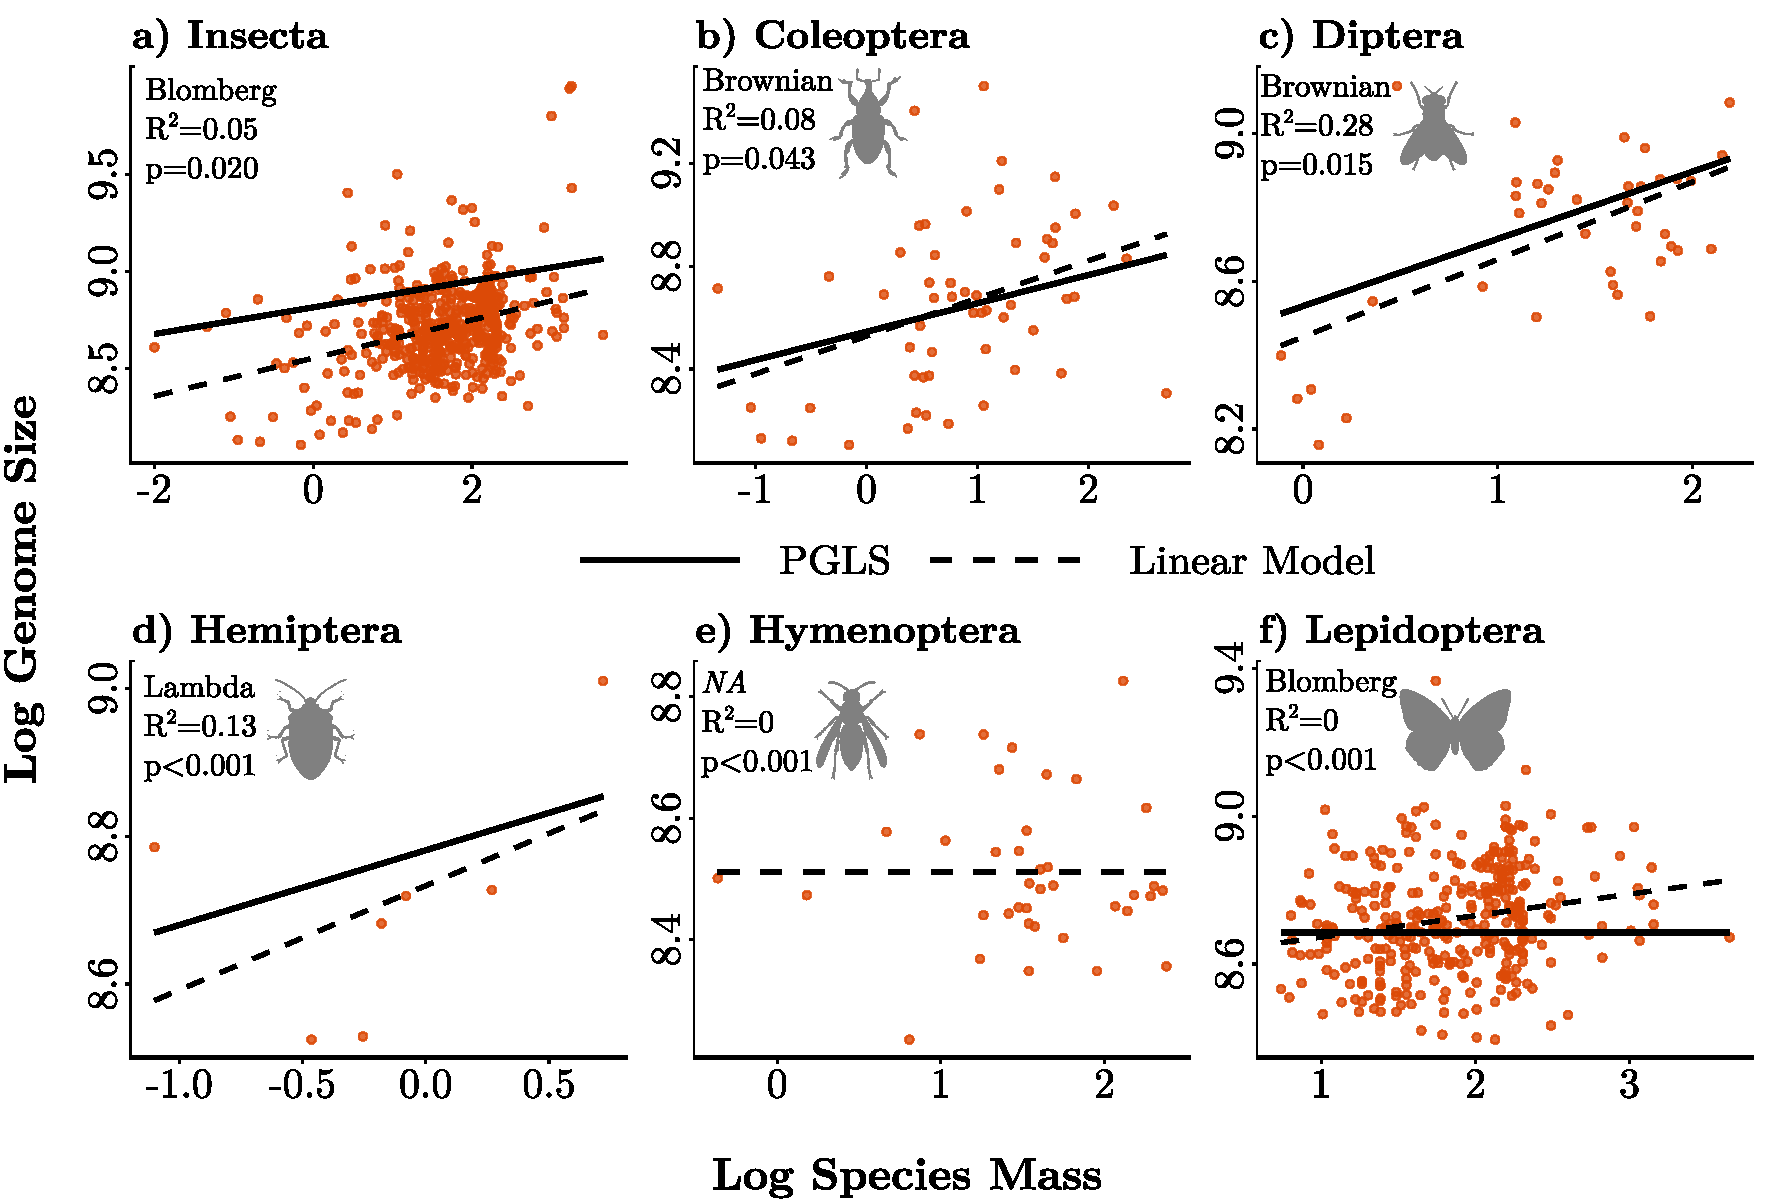
\includegraphics[width=0.92\textwidth]{figures/mass_genome_figure_orange.pdf}
    \caption{Comparison of the log10 mass of species (mg) to the log10 genome size of their assemblies. PGLS and linear regression analyses were performed in all insects, across 11 orders, (\textbf{a}) and individual orders (\textbf{b-f}). Linear regression models were performed without phylogenetic correction. Specific PGLS error structures, significance values and pseudo--$R^2$ values are detailed in the individual panels.}
    \label{fig:genome-mass-figure}
\end{figure}
\pagebreak


\subsection{Gene loss is linked to body mass}
For the TOGA analyses, there are generally significant trends of gene loss relative to mass across order and metric (see Figure~\ref{fig:toga-mass-figure}). All orders showed a significant negative trend in at least one gene loss metric: number of One-to-None genes in Coleoptera, Hymenoptera, and Lepidoptera, and One-to-None Ratio in Coleoptera and Diptera. For I/PI, there is a slight positive relationship in the number of intact \& partially intact genes in Coleoptera, but the trend is not visible or significant in other orders.


\begin{figure}[h]
    \centering
    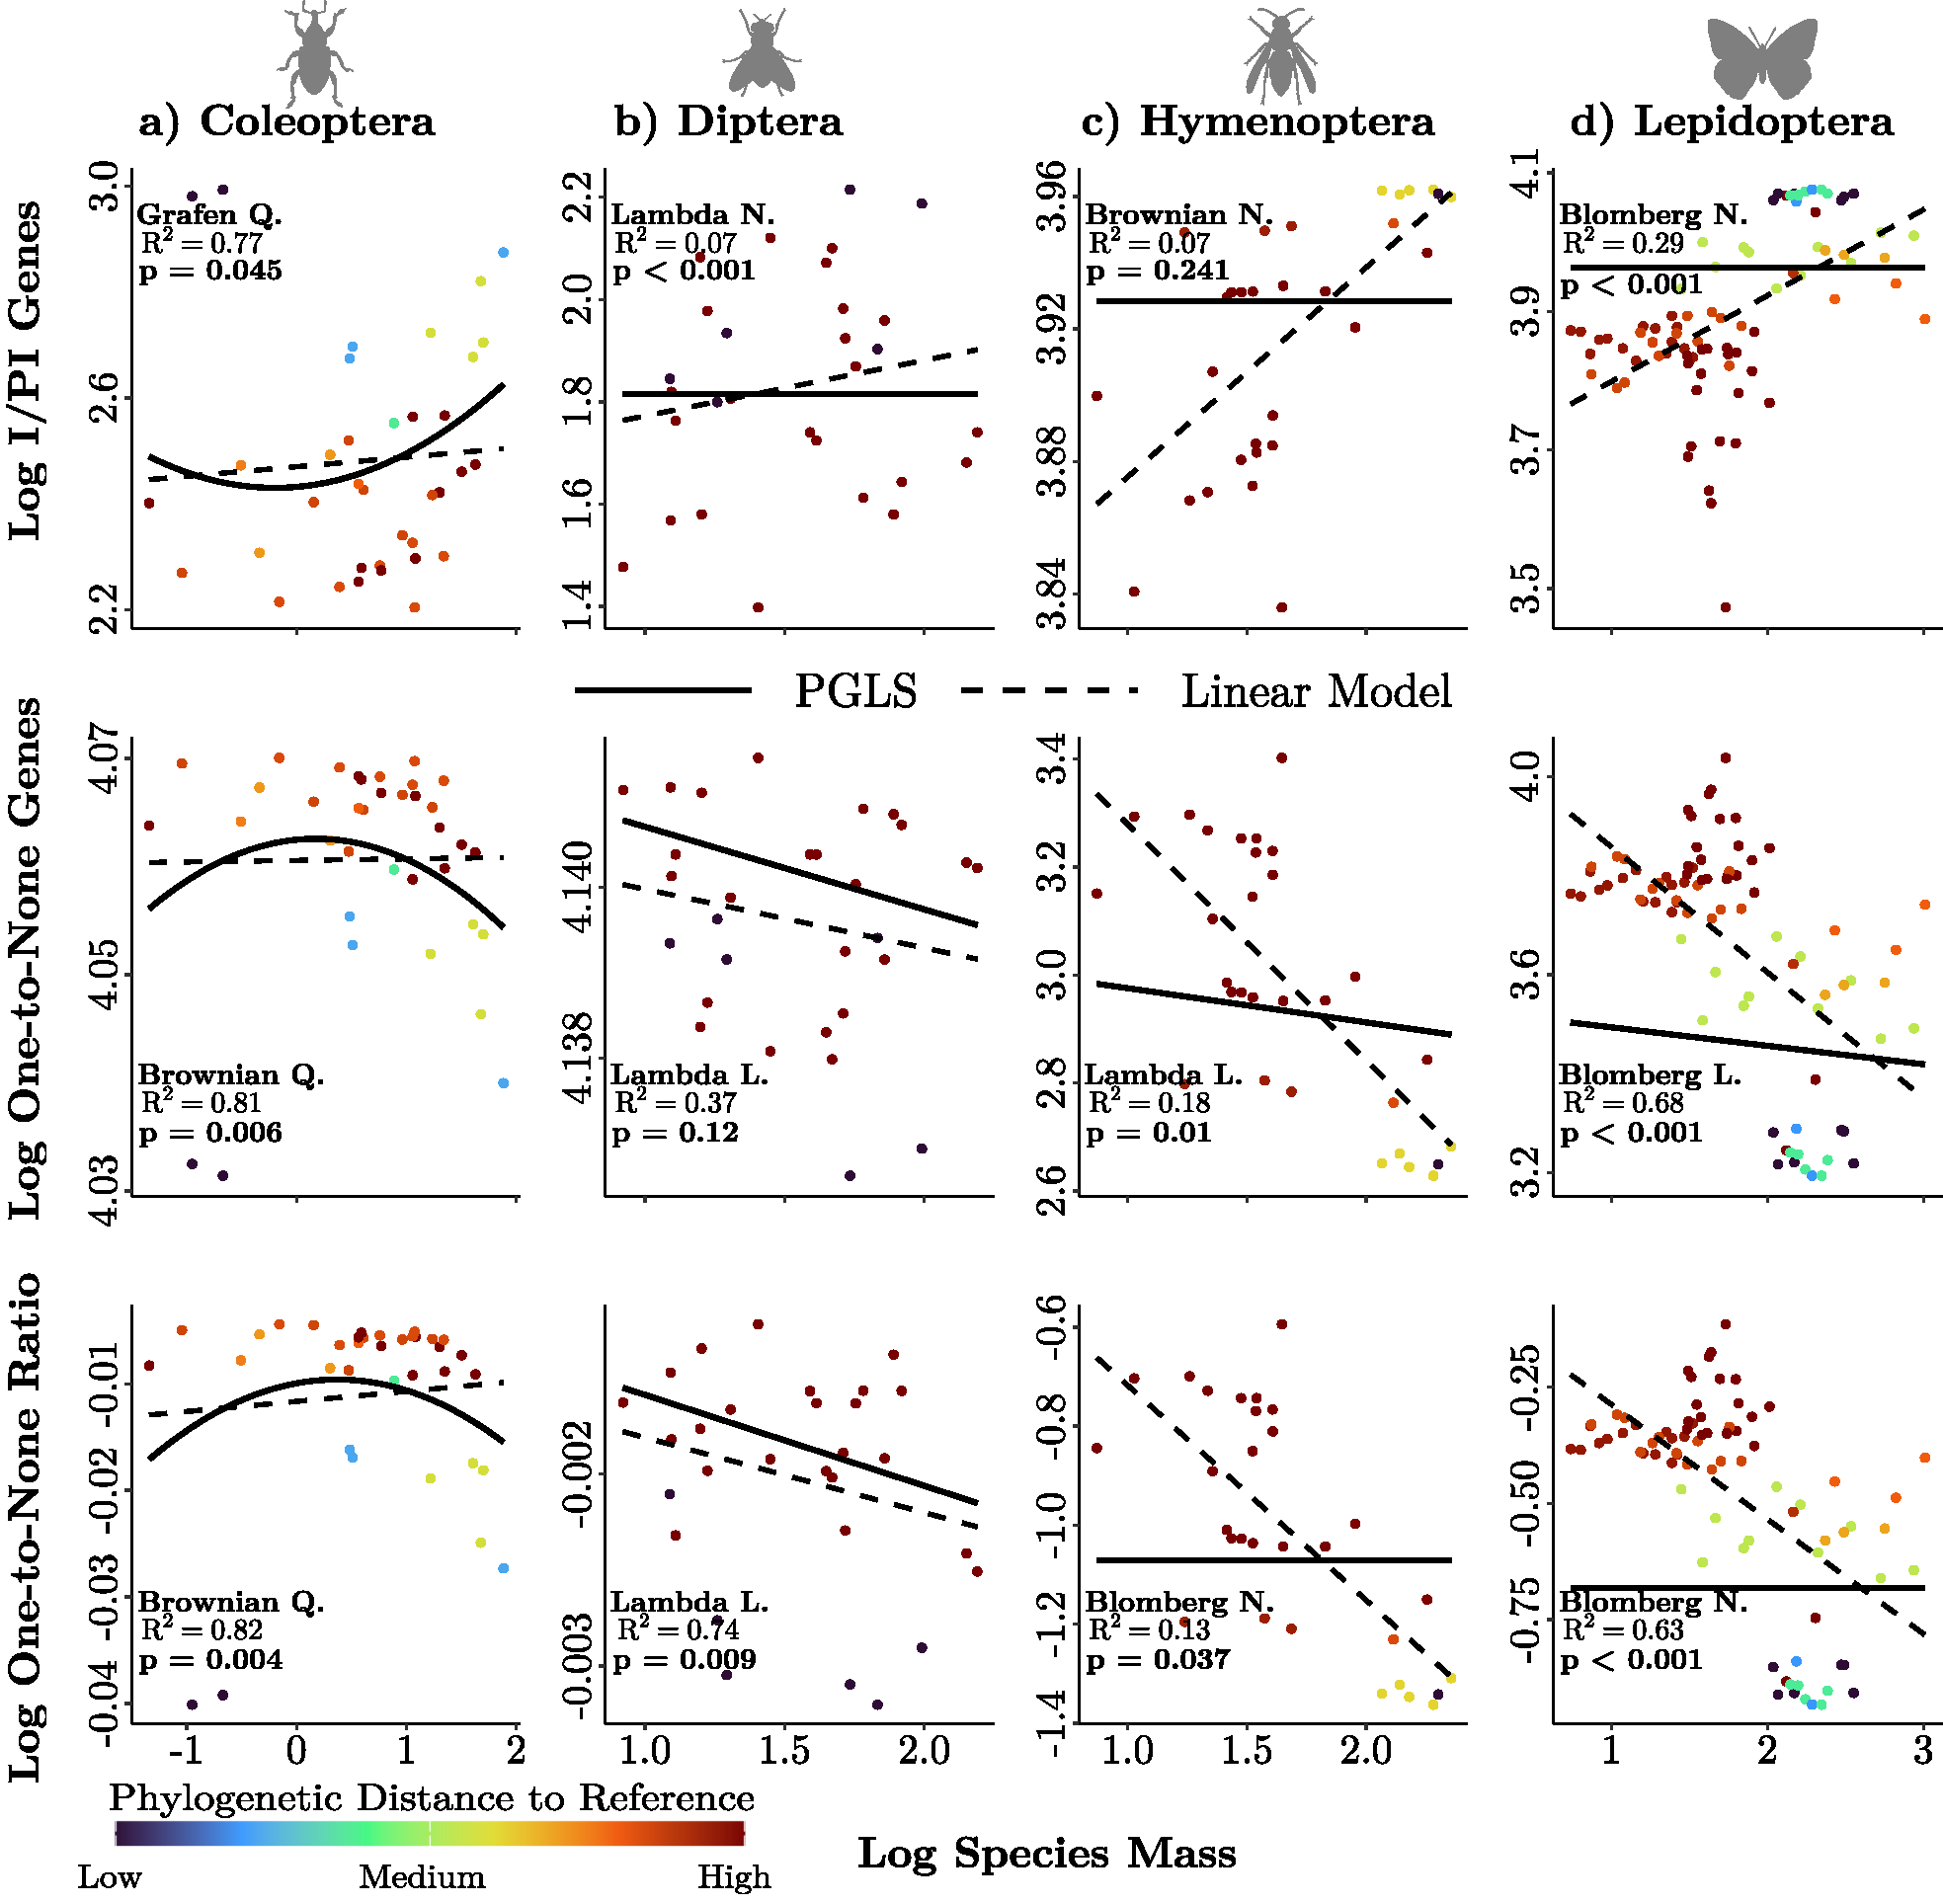
\includegraphics[width=0.95\textwidth]{figures/TOGA_Output_Final_with_illustrations.pdf}
    \caption{Relationship between the log10 mass of species (mg) and log10 gene loss metrics obtained from TOGA analyses. Columns represent each insect order (\textbf{a--d}), while rows display each loss metric examined across orders. Phylogenetic distance was included as an independent variable in all models to account for bias in gene identification (see Methods 2.3), and is visualised here in colour. For details on the variables used, refer to Methods 2.2. Figure contains the PGLS error structures, significance values, pseudo--$R^2$ values, and best model type: null (\textbf{N}), linear (\textbf{L}) or quadratic. (\textbf{Q})} 
    \label{fig:toga-mass-figure}
\end{figure}
\pagebreak

\subsection{Body mass affects some Hox genes}
\noindent The analyses performed on the number of Hox genes per family and on the total number of Hox genes per species revealed a consistently non-significant relationship with log body mass across and within all insect orders (see Figure \ref{fig:hox_gene_figure}). However there were two exceptions to this, where in the comparison of all insects the number of \textit{rough} (\textit{Ro}) and \textit{caudal} (\textit{cad}) genes per species was significantly influenced by log body mass. Although both models showed a significant difference ($>2$) in their AIC scores compared to the null model ($\Delta\text{AIC}_{Ro} = 17.2$; $\Delta\text{AIC}_{cad} = 44.4$), their $R^2$ values indicated a poor explanation of the variance in the data. Non-significant findings from all other insect orders can be seen in Supplementary Information~4.
% \vspace{0.5cm}
\begin{figure}[!b]
    \centering
    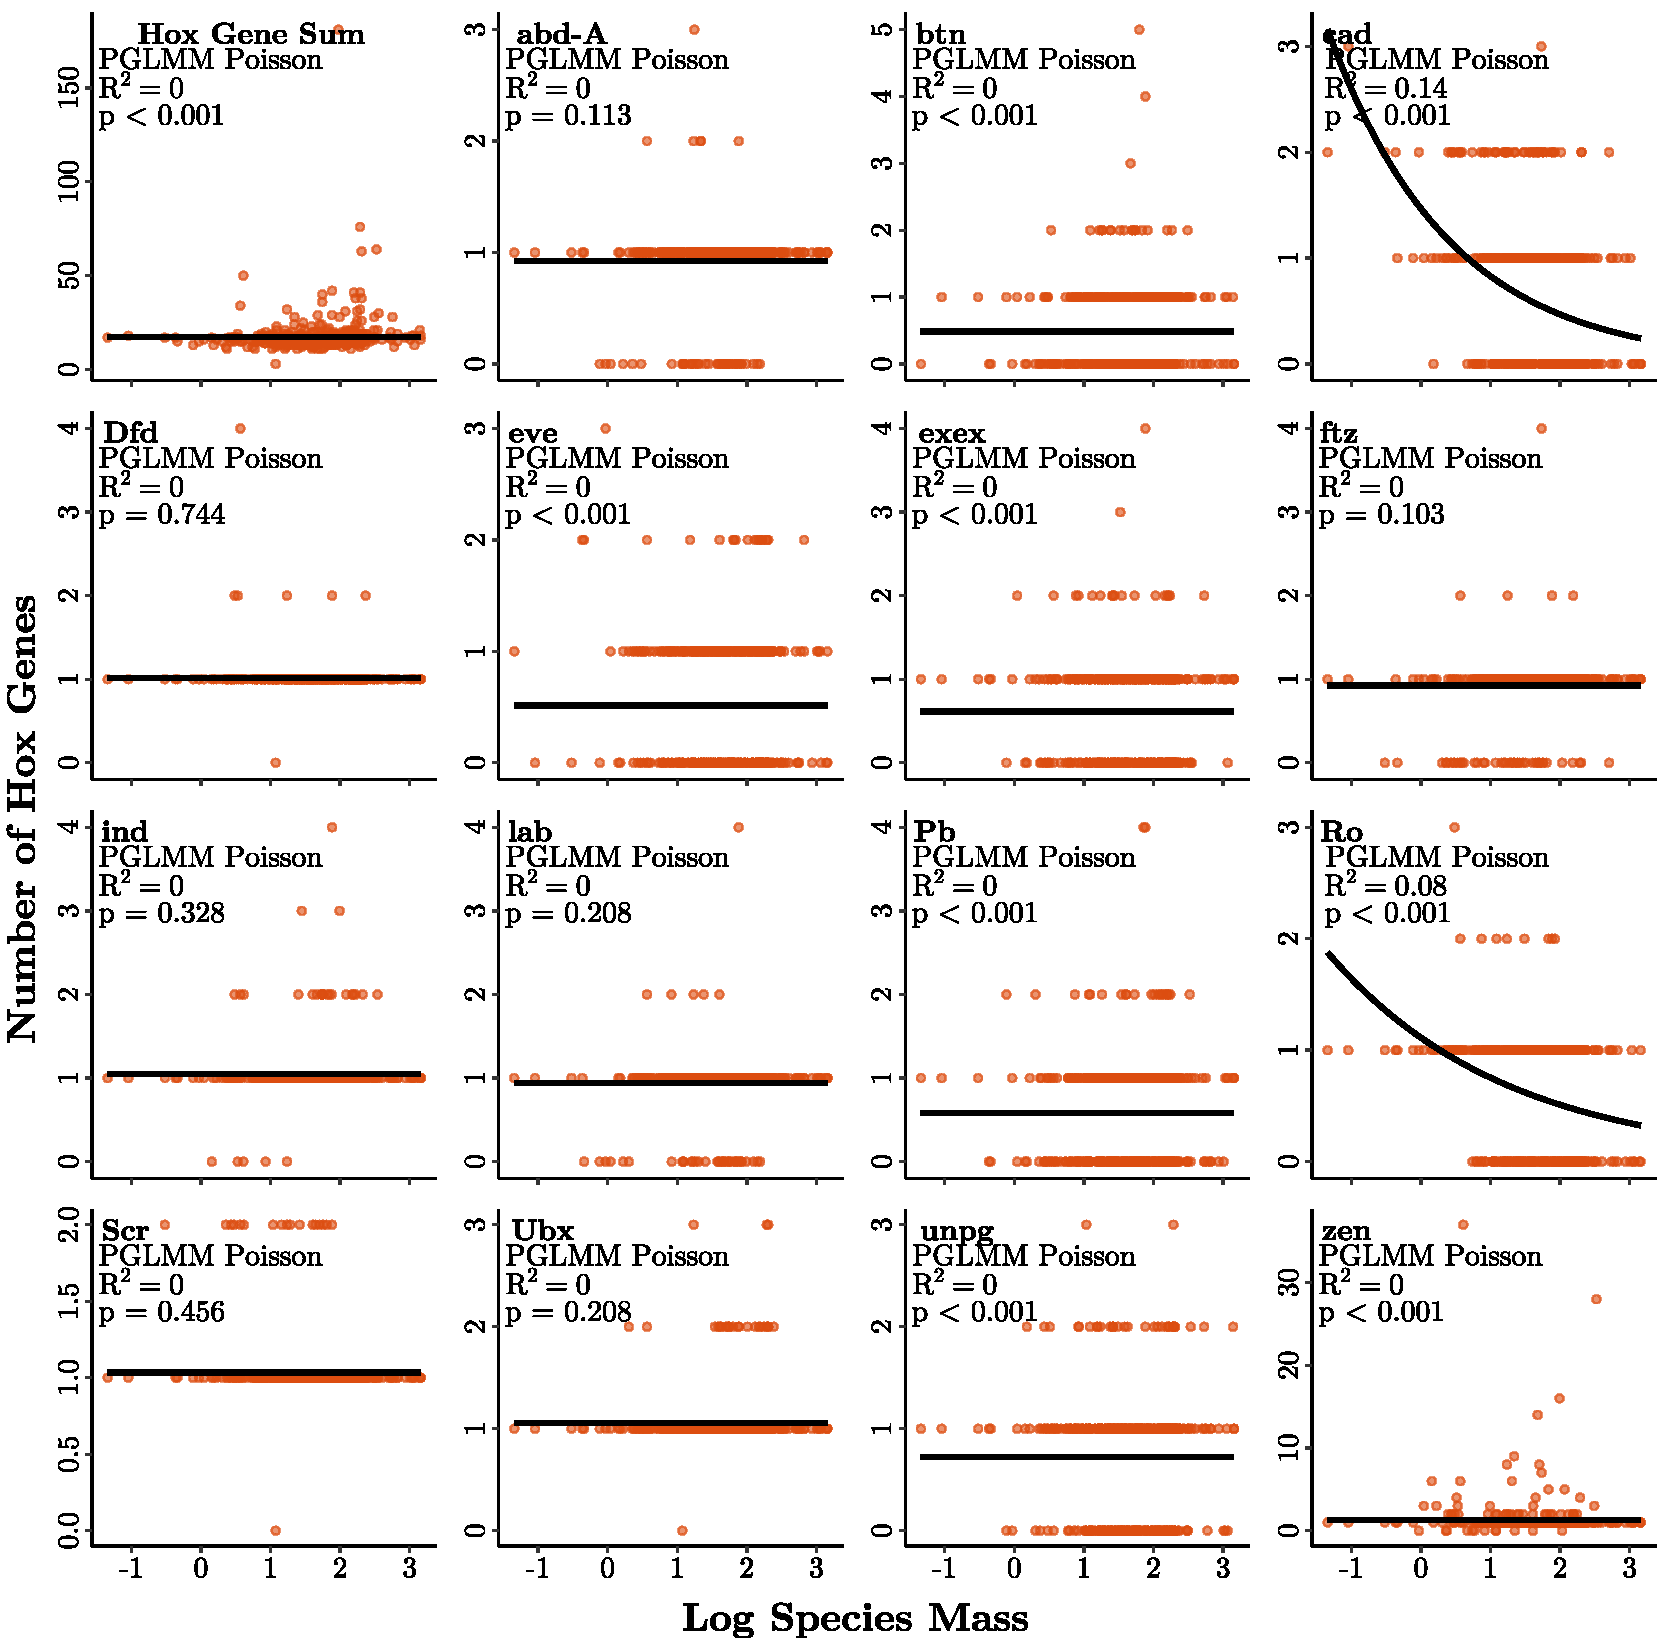
\includegraphics[width=0.93\textwidth]{figures/hox_gene_analysis_insecta.pdf}
     \caption{PGLMM predictions for number of Hox genes per species against log10 species mass (mg) estimated from Poisson models across the entire insect sample set. Hox gene name, pseudo--$R^2$ and p--values included in each panel. See Supplementary Information~4 for the non-significant results in genes within individual orders.}
    \label{fig:hox_gene_figure}
\end{figure}
\pagebreak


\vspace{1cm}
\subsection{Transposable elements scale with body mass in some orders}
The analyses assessing the relationship of body mass with the proportion of transposable elements in the genome generally showed a lack of influence of body mass on TE length, visible in Figure \ref{fig:te-mass-figure}. In all cases, the PGLS analyses with a Lambda error correlation structure fit better than non-phylogenetically controlled linear models and other PGLS' with different error structures; however, many were non-significant. There was only a significant relationship in the Coleoptera and Hemiptera, with the former showing a moderate explanation of the overall variance and the latter minimal (PGLS with Lambda structure; $p<0.001$, $R^2 = 0.53$ and $p<0.001$, $R^2 = 0.17$, respectively).

\vspace{1.5cm}
\begin{figure}[!h]
\centering
    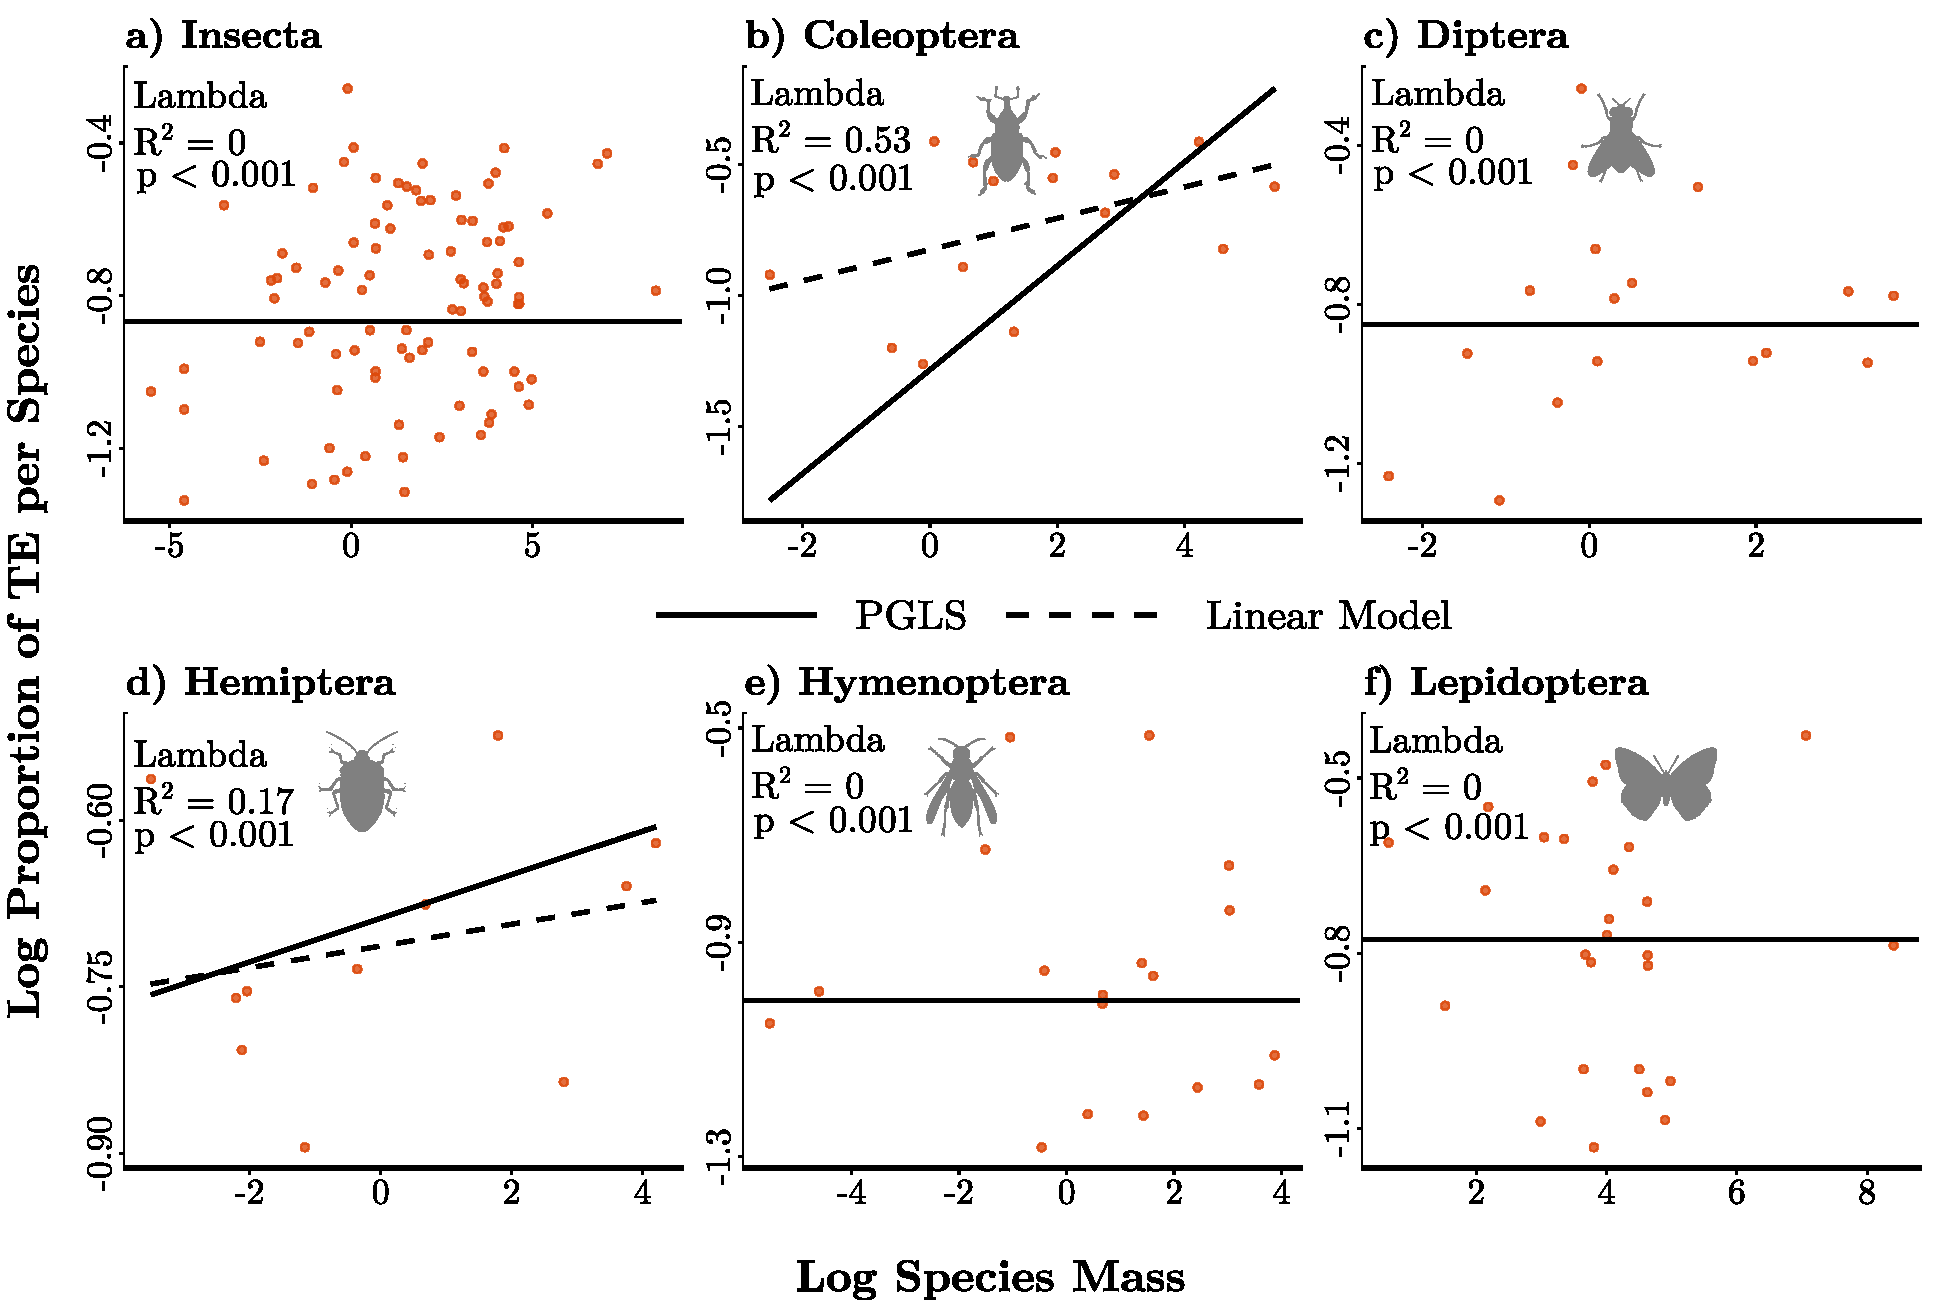
\includegraphics[width=0.95\textwidth]{figures/TE_mass_orange.pdf}
    \caption{Comparison of log10 mass of species (mg) to the log10 proportion of transposable elements (TE) in their genome. Models were fit across all insects (\textbf{a}) and individual orders (\textbf{b-f}). Simple linear regression models were fit without phylogenetic correction, and null PGLS visualised as the intercept of the null PGLS model when it was the best fitting model. Data on transposable elements was obtained from \cite{600TEs}.}
    \label{fig:te-mass-figure}
\end{figure}
\justifying

\clearpage
\pagebreak


\section{Discussion}
In this study, I sought to address three specific hypotheses regarding the coevolution of insect genomes and their mass. In the first part, I assessed whether larger species exhibit larger genome sizes. Here, I show a significant relationship between insect body mass and genome size when including 11 orders of insect, that has not been previously identified \citep{propagule}. Within orders, the findings in Coleoptera and Hemiptera contradict the existing literature that suggests that there is no relationship within these orders. The weak positive correlation suggests a link between the DNA content of a cell influencing the size of the organism, possibly indicating that a larger genome is, minimally, necessary to support the increased metabolic and structural demands with increased size. Thus, larger genomes may provide increased genetic capacity for the development and maintenance of more complex body structures and metabolic pathways. However, \cite{propagule} questioned this with their recent research in crustaceans, a group within invertebrates alongside insects, suggesting that propagule size (egg and/or sperm) correlates better than body size with genome size. This is because larger genomes often lead to larger cell sizes and because invertebrate life begins at the single cell, it is more likely to be influenced by genome size. \cite{insect-egg-genome} found contradictory results in their study of insects, in which egg size did not correlate with genome size; however, their study includes relatively small and uneven sample sizes across orders, likely skewing their comparisons.

There are two exceptions where larger insects do not have larger genomes: Hymenoptera and Lepidoptera. This indicates a more complex relationship between genome size and mass, with different eco-evolutionary forces at play. In Hymenoptera, social organisation may influence genome evolution. For example, eusocial bees and wasps have smaller genomes than their non-eusocial counterparts \citep{termite-eusociality, shrimp-eusociality}. As eusocial insects share reproductive labour, they have a reduced effective population size, making them increasingly vulnerable to invasions of deleterious mutations from mobile genetic elements \citep{eusociality-Ne}. Their smaller genome size is maintained through increased genetic recombination \citep{eusociality-recombination}, where genetic material is exchanged along or between chromosomes, breaking the coding sequences of mobile genetic elements, and prohibiting the introduction of deleterious mutations \citep{hymen-recomb-1, hymen-recomb-2}. In Lepidoptera, species life history may obscure genome size-mass trends. Specifically, development rate is negatively correlated with the genome size of some moth families, but not in others \citep{lep-genomes2}. Additional effects come from feeding preferences, where polyphagous stem borers have much longer genomes than monophagous species \citep{polyphagous-leps}. Generally, traits such as development rate, host-plant specificity, and feeding preferences are phylogenetically-correlated traits \citep{leps-phylogeny}. This indicates the need to study the evolution of the lepidopteran genome at closer taxonomic levels, to avoid the confounding effects of ecological traits. Such practices should be applied to the study of all insect orders, as these downfalls of comparative genomic analyses exist throughout the insect tree of life \citep{arthropod-gs-phylogeny}. 

I also investigated whether there were patterns of gene loss associated with size. I find a negative relationship between gene loss and body mass in a metric of gene loss, with fewer functional genes found as body mass increases. This result challenges my initial hypothesis that suggests there should be a greater number of genes as body mass increases. I constructed my hypothesis on the basis of bacterial systems and eukaryotic complexity. The number of genes in the bacterial genome is expected to increase proportionally to size, because bacterial genomes are highly specialised in function and the volume of bacterial cells limits the capacity a genome can occupy \citep{DeLong}. Furthermore, the increase in the number of unique adaptations for multicellular organisms is believed to require increased genomic complexity to encode structure and function \citep{genomecomplexity, bingham}, and the need for more structure will increase with size due to nonlinear scaling of surface area-to-volume ratios \citep{ruppert1983morphology, system-scaling}. My findings contradict these expectations and suggest a different evolutionary trajectory in which gene loss is more crucial in the evolution of body size. 

The observation that gene loss could play an important role in body size evolution challenges traditional views of genome evolution, whereby gene loss has long been assumed to be a neutral process in which redundancy decreases with little evolutionary change \citep{evolution-by-gene-loss}. Instead, it aligns with the broader framework of genome streamlining theory, suggesting that gene loss can act as a method to increase genome architecture efficiency by removing redundant or unnecessary functional gene networks \citep{olson}. In the specific case of gene loss and body size, rather than larger organisms requiring an increased number of genes to support more robust body structures and complex metabolic pathways, genome streamlining suggests that a more efficient genome will facilitate species adaptation to ecological niches that favour certain life histories \citep{genome-streamlining}, and in this case a larger body size. For example, in some \textit{Drosophila} fly species, the loss of odorant receptor genes has facilitated their expansion into new ecological niches, with associated losses of behaviour and newly obtained diets \citep{drosophila-gene-loss}. Although examples like this illustrate genome streamlining along a shorter evolutionary time frame, it is unclear whether this mechanism explains the macroevolutionary findings of this study.

A second possible mechanism of gene loss is that of regressive evolution. Loss of use of a trait puts the genes that encode it under weaker selection and allows mutations that ultimately stop gene function to accumulate \citep{evolution-by-gene-loss}. Regressive evolution often occurs in species that have either transitioned into new ecological niches or experienced environmental changes that render previously useful traits obsolete. Examples of regressive evolution include flightless birds and cave-dwelling species \citep{cave-dwelling-flight}, such as dytiscid water beetles in aquifers losing eye pigment genes due to the lack of light in their environment \citep{cave-beetles}. In the context of the correlation of body size and gene loss, regressive evolution suggests that genes encoding ecologically essential functions in smaller species become redundant as they adapt to niches that favour larger size and will be lost over time. Regressive evolution, genome streamlining, or a combination of the two could be the mechanism responsible for the resulting trends of gene loss in this analysis.

Furthermore, my analysis of the number of Hox genes indicated a decrease in the number of caudal (\textit{cad}) and rough (\textit{Ro}) genes alongside increase in mass. These genes are critical in the development of the anal plates and sensory mechanisms of the posterior region of the insect body, and photoreceptors in the eye, respectively \citep{rough, caudal}. Despite the statistical significance of this finding, the lack of biological reasoning for these genes being affected by mass and the low $R^2$ values indicate a weak correlation that may be induced by technical or statistical errors. This is reinforced by my finding that these genes have been lost in many species, which is known to cause detrimental effects to their development, though studied in individual organisms and not across species \citep{rough, caudal}. In addition, these findings are only significant when the pattern is examined across all insects and not within orders. Thus, these results likely do not represent true evolutionary trends, but are the result of inaccurate gene loss detection. The lack of consistent findings in the broader Hox gene analysis, considering both within and between insect orders, suggests that body size evolution may be influenced by genomic factors further than traditional developmental pathways. Although Hox genes play a crucial role in the development of the insect body plan \citep{hox-length}, my analyses suggest that other genetic elements, possibly related to metabolism, growth regulation, or non-coding regions, could be responsible in driving the relationship of gene loss in the evolution of body size. 

My final hypothesis proposed that larger organisms should have more non-coding DNA. I studied this in the form of transposable elements because they are well documented and there is considerable available data on their accumulated proportion in insect genomes \citep{600TEs}. My hypothesis was based on the theory by \cite{Kozlowski} that non-coding DNA is linked to body mass through the effect that genome size has on cell size. Higher accumulation of non-coding DNA leads to larger genomes and larger cells to support this \citep{cavalier-smith}, with lower metabolic rates as an inherent advantage of this and, in turn, increased body mass \citep{DeLong, glazier-cell-metabolic-rate}. However, the results from my analysis challenge their conclusions, indicating that across insects there is no clear link between body size and non-coding DNA. The discrepancy between the predictions by \cite{Kozlowski} and my findings lies in their link between cell size and body mass. Cellular metabolism of a single cell organism is closely related to its size, while organismal metabolism is more closely related to body size, which is determined by a variety of factors, including the number of cells in an organism, their methods of organisation in tissues, and the specific metabolic rates of those structures \citep{organ-metabolism}. Taking into account my findings that identified a positive correlation between genome size and body mass, as well as consistent gene loss in larger individuals, the lack of correlation of transposable elements with body size suggests that there are alternative signatures within the genome that have evolved alongside body size. If non-coding DNA is in fact correlated with body mass, it is unlikely to contain regions of non-coding transposable elements, as these seem to evolve independently of body mass when studied across all insects. 

In this study, I improve on previous literature with my use of physiological, phylogenetic, and genomic information on insects; however, my methods face a limited number of constraints that are primarily caused by my chosen method of estimating the size and complexity of the coding genome. A major limitation of TOGA is its ability to detect only gene loss and not gene gain, due to its use of existing genome annotations \citep{TOGA}. Although gene gain is less common than loss, it is possible especially on a macroevolutionary scale \citep{gene-loss-vs-gain-2, evolution-by-gene-loss, geneloss_vs_gain}. TOGA works best in pairwise comparisons, using each species as a reference, which requires annotations for all species to determine gene presence or absence. Whole transcriptomes would also allow for a similar comparative analysis \citep{transcriptome}. In the absence of such data \citep{insectbase}, computational methods could have provided approximate estimates of gene gain using stochastic simulations under evolutionary expectations, such as `CAFE'\citep{CAFE} and `BadiRate' \citep{BadiRate} software packages, but limited time did not allow for this. 

Furthermore, the overlapping mass and genomic data set includes species with different life history traits that could have impacted their rates of gene loss \citep{leps-phylogeny, arthropod-gs-phylogeny}. My analysis of genome size and body mass could have benefited from the inclusion of life-history traits; however, such data is only vastly available for limited orders of insects \citep{shirey}. Regardless, the trends identified using phylogenetically-controlled methods are strong and consistent enough that this did not hinder its ability to provide insightful results.

Finally, despite the use of transposable elements enabling the study of non-coding DNA, this methodology may potentially be a limitation of this analysis. Transposable elements are significant components of the non-coding region of genomes and are associated with genomic expansions because of their ability to insert themselves and multiply within the genome \citep{hadji-te-rna}. Although this makes them an appropriate group of non-coding DNA to study in relation to body mass, transposable elements can be actively involved in host adaptation. \cite{transposable-elements-drosophila} demonstrated that transposable elements contributed to the adaptation of \textit{Drosophila melanogaster} to temperate climates by influencing gene expression and introducing genetic diversity. The correlation between transposable elements and body mass in Coleoptera and Hemiptera may therefore indicate a more dynamic interaction of transposable elements in the evolution of mass in these orders. Although this may indicate misuse of transposable elements in this analysis, it also implies that non-coding DNA is likely more than just unnecessary excess in the genome \citep{Havstad2022-hz}, and is an important genomic factor contributing to species evolution along wider time scales.

To conclude, I identified consistent trends of larger insects having larger genome sizes, supporting the hypothesis that a larger size requires increased genomic content to encode metabolic pathways and structure. Exceptions to this rule suggest that ecological and behavioural traits, such as eusociality and feeding preferences, as well as evolutionary history, may influence genome evolution. The finding of gene loss being correlated with larger size challenges traditional views of genomic evolution and instead suggests more complex evolutionary pathways, involving genome streamlining and regressive evolution. Furthermore, the lack of a clear correlation between transposable elements and body mass indicates that genomic features further to non-coding DNA could be relevant to body size evolution in insects. Despite my study advancing the understanding of comparative genomics of insects, the limitations in detecting gene gain, use of transposable elements as a proxy of non-coding DNA, and inclusion of species with diverse life histories, regardless of their evolutionary implications, suggest areas for future research in this field. Overall, the findings presented here provide insight into the complex dynamics between genomes and morphology.

\pagebreak

\addcontentsline{toc}{section}{Code and Data Availability}
\section*{Code and Data Availability}
The code and data required for the collation of mass data are available on \href{https://github.com/icgk523/InsectMasses.git}{GitHub -- Repository 1}. \\
The remaining code and data required for repeating the data analysis and visualisation of this study are available on \href{https://github.com/icgk523/CMEE_Project.git}{GitHub -- Repository 2}.
\pagebreak

\begingroup
% \renewcommand{\refname}{\vspace*{-\baselineskip}\section{References}}
\addcontentsline{toc}{section}{References}
\bibliography{bibliography}
\endgroup



\pagebreak
\nolinenumbers

\addcontentsline{toc}{section}{Supplementary Information}
\section*{Supplementary Information}
\vspace{-0.25cm}

\addcontentsline{toc}{subsection}{SI 1: Body mass data references}
\subsection*{SI 1: Body mass data references}

Supplementary table with sources of insect size and mass used in the study. Information includes the corresponding numbers of orders and species included in the source data, as well as whether they were estimated through regressions, the trait measured, and the state of the insects at measurement.
\vspace{-0.5cm}
\singlespacing
\begin{longtable}{lccccc}
\textbf{Citation} & \textbf{Orders} & \textbf{Species} & \textbf{Regressions} & \textbf{Size/Mass} & \textbf{Live/Dry} \\
\hline
\citesuppone{coleoptera} & 1 & 2390 & Yes & Mass & Live \\
\citesuppone{kuhsel} & 4 & 113 & No & Mass & Live \\
\citesuppone{fielding} & 1 & 32 & No & Mass & Live \\
\citesuppone{bruckner} & 3 & 113 & & Mass & Dry \\
\citesuppone{kinsella} & 1 & 1054 & Yes & Mass & Dry \\
\citesuppone{horne} & 8 & 118 & No & Mass & Dry \\
\citesuppone{kendall} & 2 & 494 & & Mass & Dry \\
\citesuppone{leiva} & 8 & 123 & & Mass & \\
\citesuppone{brose} & 11 & 108 & Yes & Mass & Live \\
\citesuppone{waller} & 1 & 1011 & No & Size & \\
\citesuppone{Middleton-Welling} & 1 & 542 & No & Size & \\
\citesuppone{shirey} & 1 & 12172 & No & Size & \\
\citesuppone{Hagge} & 1 & 1157 & No & Size & \\
\citesuppone{Gillespie} & 1 & 588 & No & Size & \\
\citesuppone{white} & & & No & Mass & Live \\
\citesuppone{Ehnes} & 18 & 437 & No & Mass & Live \\
\citesuppone{Dillon} & 16 & 361 & No & Mass & Dry \\
\citesuppone{Diorhabda} & 1 & 1 & No & Mass & Live \\
\hline
\end{longtable}
\vspace{-0.75cm}

\onehalfspacing
\bibliographystylesuppone{agsm}
\bibliographysuppone{bibliography}
\pagebreak


\singlespacing

\addcontentsline{toc}{subsection}{SI 2: Conversion equations from size to mass}
\subsection*{SI 2: Conversion equations from size to mass}
Supplementary table with conversion equations used to estimate insect mass from size. Conversions varied by measurement proxy: forewing length for Lepidoptera, hindwing length for Odonata, and whole body length for other orders and suborders.
\begin{longtable}{l c l}
\textbf{Order \& Suborder} & \textbf{Mass Equation} & \textbf{Citation} \\
\hline
\endfirsthead

\multicolumn{3}{c}%
{\tablename\ \thetable\ -- \textit{Continued from previous page}} \\
\textbf{Order \& Suborder}&\textbf{Equation} & \textbf{Citation} \\
\hline
\endhead

\hline \multicolumn{3}{r}{\textit{Continued on next page}} \\
\endfoot

\hline
\endlastfoot

Blattodea &  $0.0494 \times \text{Size}^{2.344}$ & \citesupptwo{Hodar} \\
Coleoptera & $0.0389 \times \text{Size}^{2.492}$ & \citesupptwo{Sample} \\
Diptera & $0.0414 \times \text{Size}^{2.213}$ & \citesupptwo{Sample} \\
Ephemeroptera & $0.0070 \times \text{Size}^{2.880}$ & \citesupptwo{Smock} \\
Hemiptera & & \\
\quad\quad Heteroptera & $0.0084 \times \text{Size}^{3.075}$ & \citesupptwo{Sample} \\
\quad\quad Auchenorrhyncha & $0.0594 \times \text{Size}^{2.225}$ & \citesupptwo{Sample} \\
\quad\quad Sternorrhyncha & $0.0594 \times \text{Size}^{2.225}$ & \citesupptwo{Sample} \\
Hymenoptera & $0.0138 \times \text{Size}^{2.696}$ & \citesupptwo{Sample} \\
Lepidoptera & $-2.137 + 2.772 \times \text{Size}$ & \citesupptwo{Garcia-Barros}\\
Odonata & & \\
\quad\quad Zygoptera & $10^{-0.854} \times \text{Size}^{1.855}$ & \citesupptwo{Aromaa} \\
\quad\quad Epiprocta & $10^{-0.979} \times \text{Size}^{2.218}$ & \citesupptwo{Aromaa} \\
Orthoptera & $0.0488 \times \text{Size}^{2.515}$ & \citesupptwo{Rogers} \\
Thysanoptera & $0.0071 \times \text{Size}^{2.537}$ & \citesupptwo{Hodar} \\
\end{longtable}
\onehalfspacing
\bibliographystylesupptwo{agsm}
\bibliographysupptwo{bibliography}
\pagebreak

\addcontentsline{toc}{subsection}{SI 3: Data distributions}
\subsection*{SI 3: Data distributions}
In this subsection of the supplementary information, the distributions of data collated in this study can be seen in Figures 1--3, as partial justification for their log-transformation.

\vspace{1cm}

\setcounter{figure}{0}   
\begin{figure}[H]
    \justifying
    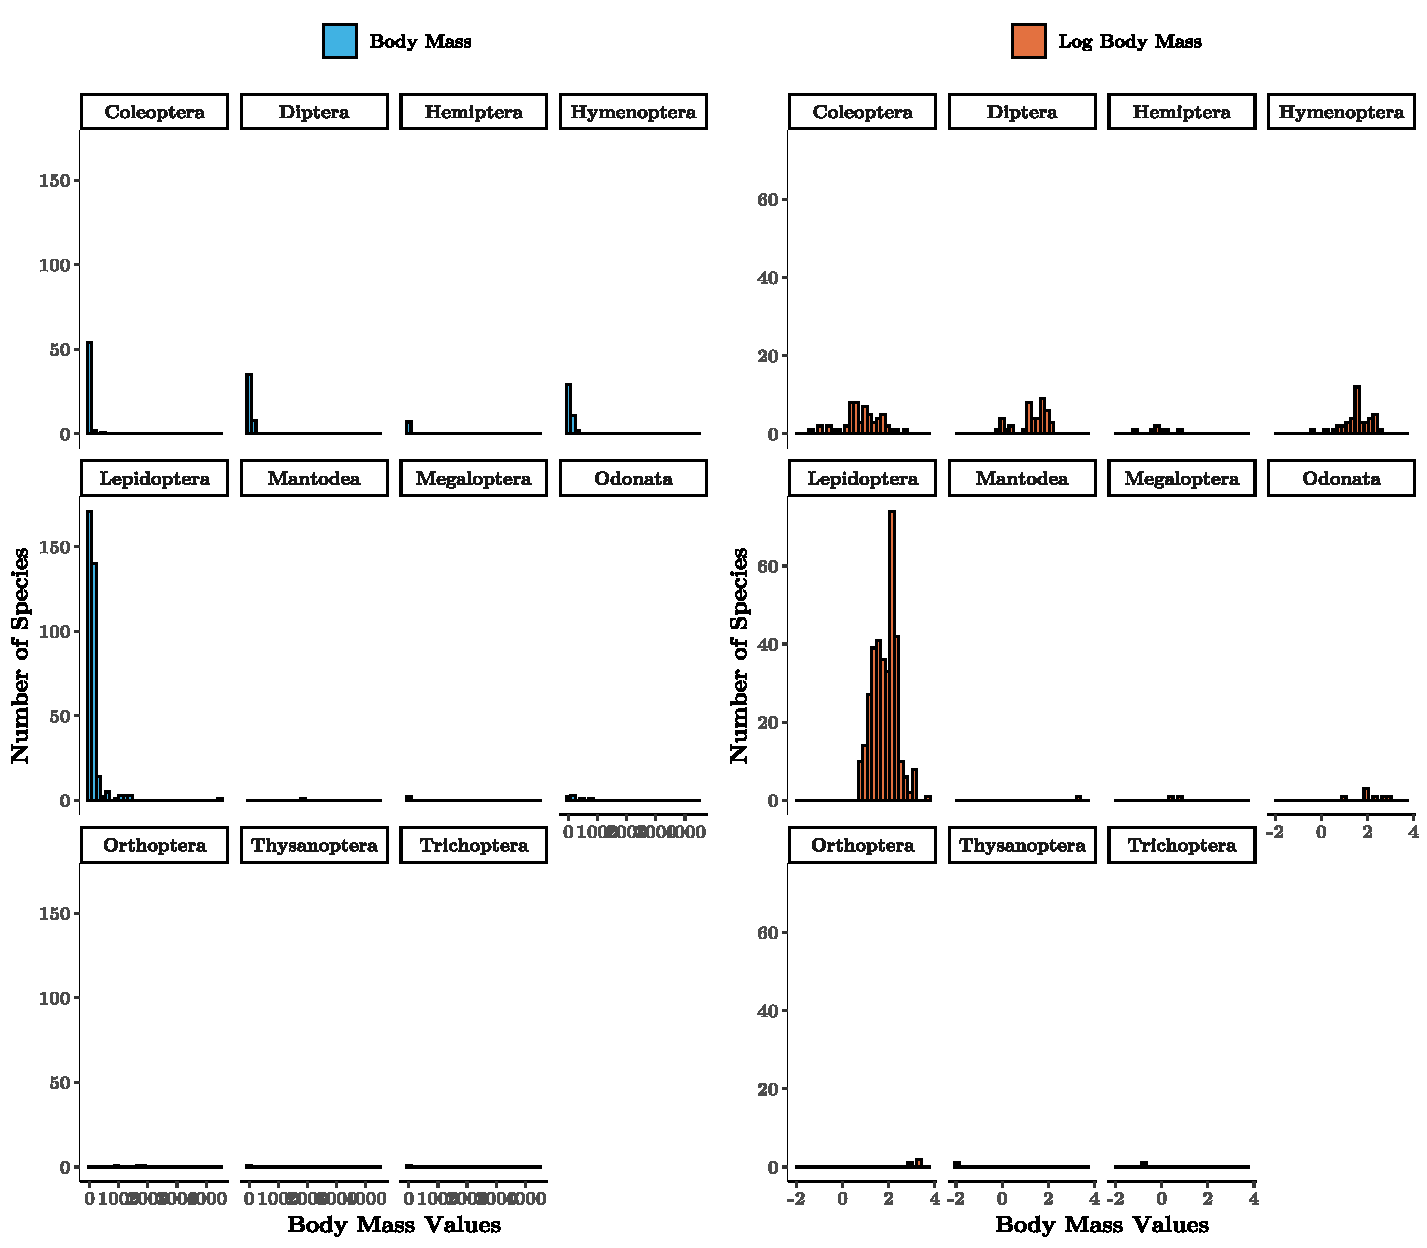
\includegraphics[width=0.9\textwidth]{figures/Mass_Distributions.pdf}
    \caption{Comparison of body mass distributions in original values (mg) and log10-transformed across orders of insects.}
    \label{fig:mass-distributions}
\end{figure}

\begin{figure}[H]
    \centering
    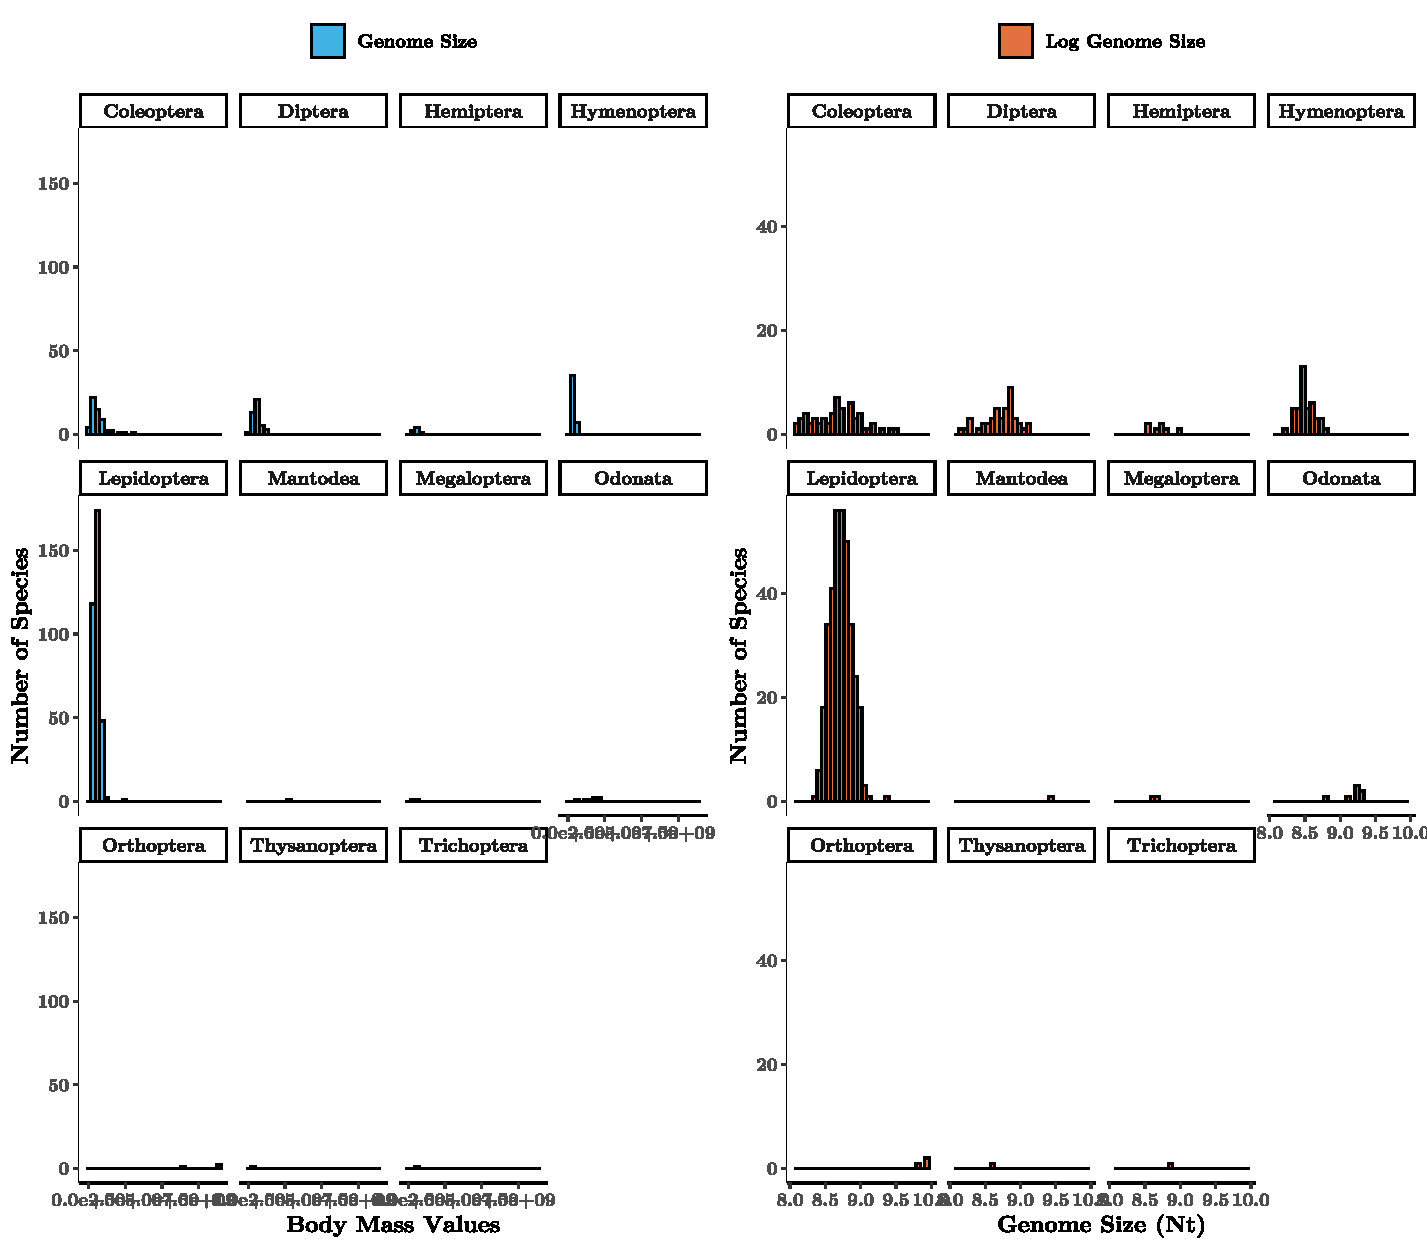
\includegraphics[width=0.9\textwidth]{figures/Genome_Distributions.pdf}
    \caption{Comparison of genome size distributions in original values (Nt -- nucleotides) and log10-transformed across orders of insects.}
    \vspace{0.5cm}
    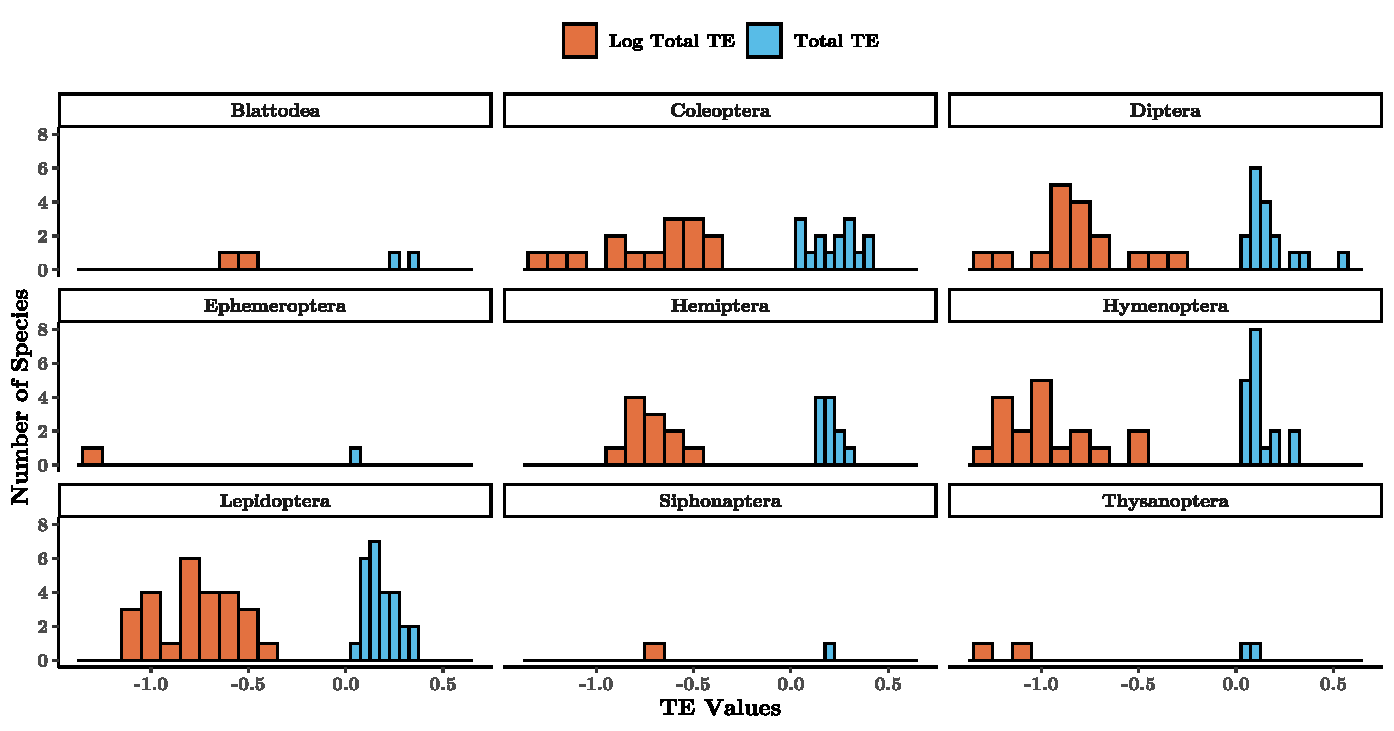
\includegraphics[width=0.875\textwidth]{figures/TE_Distributions.pdf}
    \caption{Comparison of transposable element distributions in original values (proportion of the genome~--~\%) and log10-transformed across orders of insects.}
    \label{fig:genome-te-distributions}
\end{figure}








\pagebreak
\addcontentsline{toc}{subsection}{SI 4: Expanded Hox gene analysis results}
\subsection*{SI 4: Expanded Hox gene analysis results}
Table of all Hox gene analyses for individual insect orders. All linear and quadratic models were nonsignificant following model comparisons. Information on data distributions (Poisson or Binomial), whether the models were null, linear or quadratic, p-values, and pseudo-$R^2$ values is included.
\singlespacing
\centering
\begin{tabular}{lllrrllrr}

 & \multicolumn{4}{c}{\textbf{Coleoptera}} & \multicolumn{4}{c}{\textbf{Diptera}} \\
\cmidrule(lr){2-5} \cmidrule(lr){6-9}
\textbf{Hox Gene} & \textbf{Structure} & \textbf{Model} & \textbf{$P$} & \textbf{$R^2$} & \textbf{Structure} & \textbf{Model} & \textbf{$P$} & \textbf{$R^2$} \\
\cmidrule(lr){1-9}
Abd--A & Poisson & Null & 0.888 & 0 &&&& \\
Abd--B &  &  &  &  & Binomial & Null & 0.008 & 0 \\
btn & Poisson & Null & $<0.001$ & 0 & Poisson & Null & 0.003 & 0 \\
cad & Poisson & Null & $<0.001$ & 0 & Poisson & Null & 0.874 & 0 \\
Dfd & Poisson & Null & 0.671 & 0 &  &  &  &  \\
eve & Poisson & Null & 0.002 & 0 & Poisson & Null & 0.874 & 0 \\
exex & Poisson & Null & 0.003 & 0 & Poisson & Null & 0.752 & 0 \\
ftz & Binomial & Null & 0.999 & 0 & Poisson & Null & 0.752 & 0 \\
ind & Poisson & Null & 0.888 & 0 & Poisson & Null & 0.527 & 0 \\
lab	& Poisson & Null	& 0.888 &	0	&Binomial&	Quadratic &	0.155&	0.05\\
Pb	& Poisson & Null	& 0.017&	0		& & & &	\\	
Scr	& Poisson & Null	 & 0.258	 & 0			& & & &	\\		
Ubx	& Poisson & Null & 	0.888	 & 0				& & & &\\		
unpg & Poisson & Null & 	0.888	 & 0 & 	Binomial	 & Null & 	0.209	 & 0\\
zen	& Poisson & Null & 	$<0.001$	 & 0	 & Poisson	 & Null	 & $<0.001$	 & \\
\cmidrule(lr){2-5} \cmidrule(lr){6-9}
\textbf{Sum} & Poisson & Null & $<0.001$ & 0 & Poisson & Null & $<0.001$ & 0 \\
\cmidrule(lr){1-9}
\end{tabular}


\begin{tabular}{lllrrllrr}
 & \multicolumn{4}{c}{\textbf{Hymenoptera}} & \multicolumn{4}{c}{\textbf{Lepidoptera}} \\
\cmidrule(lr){2-5} \cmidrule(lr){6-9}
\textbf{Hox Gene}  & \textbf{Structure} &  \textbf{Model} & \textbf{$P$} & \textbf{$R^2$} &\textbf{Structure} &  \textbf{Model} & \textbf{$P$} & \textbf{$R^2$} \\
\cmidrule(lr){1-9}
Abd--A & Poisson &Null &  0& 0 &  Poisson&Null &  0.956& 0 \\
btn & Poisson &Null & $<0.001$ & 0 &  Poisson&Null & $<0.001$ & 0\\
cad & Poisson &Null  & 	0.212 & 0 &  Poisson& Null	 & $<0.001$ & 	0\\
eve & Poisson &Null & 0.044 & 0 &   Poisson &Null	 & 	$<0.001$ & 0\\
exex & Poisson & Null & 0.009 & 0 &   Poisson & Null	 &  $<0.001$& 0\\
ftz & Binomial & Null & 0.001 & 0 & Poisson & 	Null	 &  0.783 & 	0\\
ind &&&&& Poisson &Null & 0.408 & 0\\
lab & &&&& Poisson & Null & 0.999 & 0 \\
Pb & Poisson & Null & 0.161 & 0 & Poisson & Null & $<0.001$ & 0 \\
Ro & Poisson & Null & 0.876 & 0 & Poisson & Null & $<0.001$ & 0 \\
Scr & Poisson & Null & 0.876 & 0 & Poisson & Null & 0.869 & 0 \\
ShxA &  &  &  &  & Poisson & Null & $<0.001$ & 0 \\
ShxB &  &  &  &  & Poisson & Quadratic & 0.145 & 0.07 \\
ShxC &  &  &  &  & Poisson & Linear & 0.056 & 0.01 \\
ShxD &  &  &  &  & Poisson & Null & $<0.001$ & 0 \\
Ubx & &&&& Poisson & Null & 0.225 & 0 \\
unpg & Poisson & Null & 0.876 & 0 & Poisson & Null & $<0.001$ & 0 \\
zen & Poisson & Null & 0.876 & 0 & Poisson & Null & 0.101 & 0 \\
\cmidrule(lr){2-5} \cmidrule(lr){6-9}
\textbf{Sum} & Poisson & Null & $<0.001$ & 0 & 	Poisson	 & Null	 &$<0.001$& 	0\\
\cmidrule(lr){1-9}
\end{tabular}
\doublespacing


\end{document}

